% SICACS / ICACS 2026 survey paper in Springer LLNCS format
% 40 selected references from docs/literature_refs_formatted.txt
% Compile: pdflatex paper.tex
%
\documentclass[runningheads]{llncs}
%
\usepackage[T1]{fontenc}
\usepackage{graphicx}
\usepackage{booktabs}
\usepackage{array}
\usepackage{url}
\usepackage{tikz}
\usetikzlibrary{shapes.geometric, arrows.meta, positioning, fit}
%
\begin{document}
%
\title{A Survey on Multi-Threat Explainable AI for Digital Deception Detection: DeepFakes, Fake News, and Recruitment Fraud}
%
\titlerunning{Multi-Threat Explainable AI for Digital Deception Detection}
%
\author{Harshida Joshi\inst{1}\orcidID{0009-0008-7301-4733} \and
Swati Sharma\inst{1} \and
Ashwini Kumar Jha\inst{1}\orcidID{0000-0002-6607-2168}}
%
\authorrunning{H. Joshi et al.}
%
\institute{Department of Artificial Intelligence \& Data Science,
Parul Institute of Engineering \& Technology,
Faculty of Engineering \& Technology,
Parul University, Waghodia, Vadodara, Gujarat, 391760, India\\
Harshida Joshi: Student, Artificial Intelligence \& Data Science\\
Swati Sharma: Assistant Professor (Guide)\\
Ashwini Kumar Jha: Co-Guide\\
\email{harshidhijoshi@gmail.com, swati.sharma@paruluniversity.ac.in, ashwinibjha@gmail.com}}
%
\maketitle
%
\begin{abstract}
Online deception rarely appears as a single, neat problem. A synthetic face can sit on a profile page, a rewritten news claim can travel through messaging apps, and a false job post can pressure applicants into sharing documents or money. Research communities have studied each of these threats in depth, but deployed authenticity tools still tend to treat them as separate classifiers. This survey reviews recent machine learning and deep learning literature on deepfake image detection, fake news classification, and recruitment scam detection, with particular attention to systems that expose why a decision was made. We organize the material around techniques that keep appearing in strong practical designs: EfficientNet-family convolutional backbones, Grad-CAM visual evidence, BERT-style text encoders, and LIME/SHAP local explanations. From the surveyed work, we highlight three stubborn gaps---cross-dataset brittleness, explanation treated as an afterthought, and thin coverage of recruitment fraud---and we argue for an evidence-aware multi-threat view of authenticity verification that fits communication platforms and digital-city services.

\keywords{DeepFake detection \and Fake news \and Recruitment fraud \and EfficientNet \and Grad-CAM \and BERT \and LIME \and SHAP \and Explainable AI \and Digital authenticity}
\end{abstract}
%
\section{Introduction}
Digital platforms lower the cost of publishing and raise the cost of verification. With common tools, a user can post a face that never lived, recirculate a headline that sounds official, or advertise a job that exists only to harvest identity documents. End users experience these as different social situations---looking, reading, applying---yet each event moves trust from a weak digital cue toward a human action.

Historically, the research response has been split along the same lines. DeepFake detection grew around convolutional networks trained on FaceForensics++, Celeb-DF, and related corpora, later joined by transformer hybrids. Fake news detection has migrated from bag-of-words and TF--IDF baselines to contextual transformers such as BERT. Recruitment scam research arrived later, with fewer public datasets and fewer dedicated system studies. Although the reported accuracies increased, another shortcoming became evident in practice. A score such as ``0.94 fake'' rarely helps a moderator or applicant who must act under time constraints.

Explainable artificial intelligence (XAI) tries to bridge this gap. The Grad-CAM overlays indicate which facial areas influenced the image model. LIME and SHAP allocate importance to words in news items or job advertisements. Explanations are imperfect; they can be coarse, unstable or misleading. However, they turn a bare label into something closer to usable evidence. This is the central theme of this survey: detection without evidence is incomplete for authenticity work.

\subsection{Contributions}
This study makes four contributions.
\begin{enumerate}
\item A multi-threat reading of the literature that places DeepFake, fake news, and recruitment scam research under one authenticity frame.
\item A compact taxonomy that separates threat modality, learning family, explanation style, and deployment concern (Fig.~\ref{fig1}).
\item Comparative tables connecting technique families to strengths, weaknesses, and evidence-aware module design.
\item A list of open problems that matter for communication systems and smart digital services, including robustness, explanation fidelity, and data scarcity in hiring fraud.
\end{enumerate}

\subsection{Paper Organisation}
Section~\ref{sec:method} states how the literature is organized and reviews earlier surveys. Section~\ref{sec:deepfake} covers the detection of DeepFake images. Section~\ref{sec:fakenews} covers fake news. Section~\ref{sec:recruit} discusses recruitment fraud. Section~\ref{sec:xai} discusses Grad-CAM, LIME, and SHAP in authenticity settings. Section~\ref{sec:data} summarizes the datasets and metrics. Section~\ref{sec:compare} presents comparative tables and a reference multi-threat pipeline. Section~\ref{sec:open} lists the open challenges. Section~\ref{sec:concl} concludes.

\section{Survey Method, Related Reviews, and Taxonomy}
\label{sec:method}

\subsection{Scope and Selection Logic}
The survey is narrative rather than a full PRISMA-style meta-analysis. We privileged peer-reviewed journal and conference papers (roughly 2020--2026) that (i)~propose or review detectors for one of the three threats, or (ii)~study the explainability of those detectors. Special weight was given to EfficientNet/CNN image work, BERT text work, and Grad-CAM/LIME/SHAP explanations because these families currently offer a realistic accuracy--cost--interpretability balance for prototype platforms. From the conducted literature collection we retain \textbf{40} technique-aligned works for this conference survey. Purely sociological scam studies are used only where they clarify threat context.

\subsection{Earlier Survey Work}
Mirsky and Lee provided a foundational account of DeepFake creation and detection~\cite{r18}. Later reviews have detailed modern models, datasets, and evaluation pitfalls, including domain shifts under new generators and compression~\cite{r08,r09,r20,r23}. Fake news surveys map content-based, propagation-based, source-based, and multimodal lines~\cite{r21,r31,r34}. Cross-cutting reviews now place fake news and deepfakes in one socio-technical frame~\cite{r01}. Recruitment fraud still lacks a dense survey literature; technical progress is mainly carried by system papers such as Fraud-BERT~\cite{r38} and related job-fraud classifiers~\cite{r37}.

\subsection{Taxonomy}
Figure~\ref{fig1} summarizes the taxonomy used in this study. The work is read along four axes:
\begin{itemize}
\item \textbf{Threat modality:} DeepFake images, fake news text, and recruitment scam text.
\item \textbf{Learning family:} classical ML, CNN/EfficientNet, vision transformers/hybrids, BERT/graph--BERT.
\item \textbf{Explanation style:} none, Grad-CAM (visual), LIME/SHAP (local text), and broader design explanations.
\item \textbf{Deployment concerns:} in-domain accuracy, cross-domain robustness, class imbalance, and human review costs.
\end{itemize}

\begin{figure}
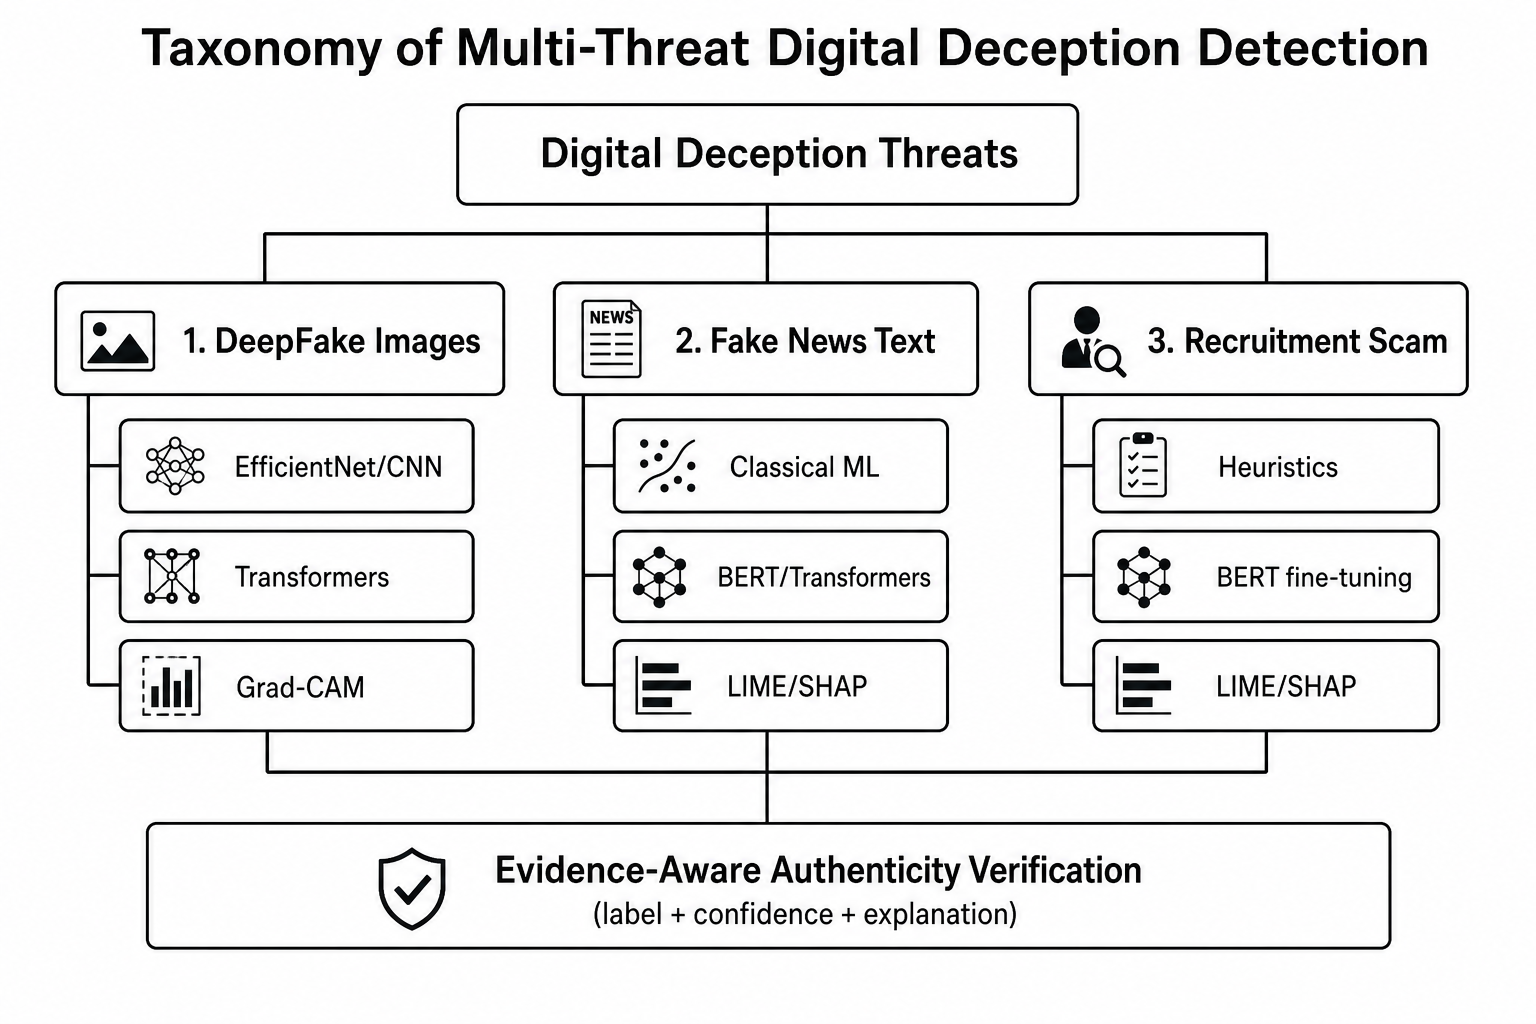
\includegraphics[width=\textwidth]{fig1.png}
\caption{Taxonomy of multi-threat digital deception detection feeding evidence-aware authenticity verification.}
\label{fig1}
\end{figure}

\noindent This taxonomy is intentionally engineering-oriented. It asks what a platform builder should choose, not only how publishers group the keywords.

\section{DeepFake Image Detection}
\label{sec:deepfake}

\subsection{Threat Setting}
DeepFake systems synthesize or edit facial images. Typical attacks include face swapping, expression reenactment, attribute editing, and fully generated portraits. Early detectors searched for blending boundaries and texture irregularities. As generators improved, these cues weakened, and models had to learn subtler inconsistencies in color, frequency response, and identity coherence.

\subsection{CNN and EfficientNet Approaches}
Convolutional networks remain attractive for still-image screening because they are mature, relatively inexpensive at inference, and easy to couple with Grad-CAM. EfficientNet variants are common because the compound scaling of depth, width, and resolution often yields a better accuracy--parameter trade-off than older heavy CNNs. Kumar et al.\ combine spatial and frequency cues around an EfficientNet backbone with attention and Grad-CAM, reporting very high AUC in controlled tests~\cite{r02}. Deepa et al.\ compared classical texture pipelines against EfficientNet-B3 and InceptionV3; deep models win clearly, with EfficientNet-B3 near 98\% accuracy in their setting~\cite{r04}. Lite CNNs and synthetic-data expansion appear when labelled forgery sets are small~\cite{r12}. Ensemble and multi-stream designs further attempt to reduce overfitting to one forgery style~\cite{r05,r17}. CNN--Grad-CAM comparisons across EfficientNet-class backbones further support explainable image screening~\cite{r39}.

For prototypes and edge-friendly services, EfficientNet-B0 is often preferred over its heavier counterparts. Larger variants may win leaderboard accuracy, but authenticity platforms also care about latency and the clarity of the accompanying heatmap.

\subsection{Transformers and Hybrid Vision Models}
Vision transformers and CNN--transformer hybrids aim to capture long-range cues that local convolutional layers miss. Convolutional vision transformers and CSWin-style systems report high accuracy on FaceForensics++/Celeb-DF-style splits~\cite{r10,r06}. Survey comparisons place some hybrids in the high 90s for accuracy on standard partitions~\cite{r09}. Contrastive and generalization-oriented DeepFake work also stresses robustness beyond a single forgery family~\cite{r11,r16}. Repeated caution is cross-condition fragility: change the generator, compression setting, or identity distribution, and the scores often fall~\cite{r08,r09}. Social uploads rarely resemble clean benchmark cuts.

\subsection{Explainable DeepFake Detection}
An operational review requires more than a probability. Platform-style systems attach Grad-CAM heatmaps and short notes for face-swap and face-generation cases~\cite{r07}. Other CNN studies reported F1 scores of approximately 0.8--0.9, depending on the architecture and data, while analyzing internal decisions~\cite{r13}. Reviews of multimodal explainable DeepFake detection argue that explanation quality must be measured, not assumed~\cite{r14}. Hybrid forged-face CNN work and quantitative XAI stress tests further motivate careful explanation validation~\cite{r15,r19}.

\paragraph{Section takeaway.}
For image authenticity services, EfficientNet-family CNNs plus Grad-CAM currently offer one of the most practical balances of accuracy, cost, and visual evidence.

\section{Fake News and Online Misinformation Detection}
\label{sec:fakenews}

\subsection{Scope and Classical Baselines}
Fake news work covers fabricated articles, misleading headlines, rumors, health claims, and low-resource or multilingual settings. Early detectors used TF--IDF, linguistic markers, SVM, Random Forest, and stacking ensembles~\cite{r21,r24}. These remain useful as transparent baselines or when labelled data are scarce, but they weaken when the same claim is paraphrased or translated.

\subsection{BERT and Transformer-Based Detectors}
Contextual transformers have reshaped this field. LSTM--BERT hybrids, dual-stream BERT--GNN models, graph-augmented ensembles, reinforced transformer designs, and transfer-learning pipelines report mid-to-high 90s accuracy on popular English corpora~\cite{r25,r27,r32,r33,r36}. Graph components are useful when interaction structure is available. Data scarcity still limits many languages; LLM-based augmentation can enlarge training sets, although synthetic text may inject its own bias~\cite{r03}. Ensemble deep models further improve in-domain performance~\cite{r28}. Broader machine-learning surveys continue to map technique and tooling choices~\cite{r30}.

\subsection{Explainable Text Classification}
High accuracy alone does not satisfy an analyst who must justify flags. BiLSTM-LIME designs show that strong scores and local word highlighting can coexist, with reported accuracy near 97\% in one recent study~\cite{r26}. BERT-oriented pipelines with SHAP have been applied to COVID-19 related claims~\cite{r40}. Reasoning-based multimodal explainable detectors and design-science evaluations of disinformation tools warn that explanations do not automatically raise trust; they can also create hesitancy~\cite{r22,r29,r35}. Therefore, LIME and SHAP are best treated as decision support, not as automatic proof of intent.

\paragraph{Section takeaway.}
BERT-family encoders are the default text backbone, and LIME and SHAP are the most common local evidence layers for word-level justification.

\section{Recruitment Scam and Employment Fraud Detection}
\label{sec:recruit}

\subsection{Why Recruitment Fraud Is Not Just Another Spam Task}
A fake job can share lexical patterns with spam or fake news, but the user journey differs. Victims may pay fees, share bank details, or send identity documents urgently. Useful signals include unrealistic salary promises, vague company identity, odd contact channels, pressure language, and severe class imbalance between genuine and fraudulent posts.

\subsection{Learning-Based Detectors}
Naud\'{e} et al.\ apply machine learning to fraudulent job-type detection and discuss social implications of algorithmic screening~\cite{r37}. Fraud-BERT fine-tunes BERT on EMSCAD-style data, where fake ads are a minority class, reporting high accuracy and strong AUC while handling imbalance better than older TF--IDF pipelines~\cite{r38}.

\subsection{Relative Immaturity}
Compared with fake news, recruitment fraud offers fewer public benchmarks, less standardized evaluation, and little systematic XAI. Therefore, method transfer is attractive: reuse BERT + LIME/SHAP from news detection, then add hiring-specific heuristics and imbalance-aware training.

\subsection{Phase-1 Prototype: Documented Heuristic Baseline}
\label{sec:recruit_proto}
To make recruitment screening auditable before journal submission, we implemented and evaluated an interpretable rule-based baseline (not a fine-tuned BERT model). The module starts from a neutral fraud prior of 50, adds or subtracts fixed weights when text, employer, and domain signals fire, clamps the result to $[8,92]$, and reports an \emph{authenticity score} $\text{trust}=100-\text{fraud}$. Posts with $\text{fraud}\geq 50$ are labeled fake; website status is \emph{Trusted} only when the employer matches a reference list \emph{and} $\text{trust}\geq 65$.

Table~\ref{tab:recruit_rules} lists every rule and weight. Figure~\ref{fig:recruit_flow} summarizes the decision order. Weights follow indicators emphasized in Fraud-BERT/EMSCAD-style work~\cite{r38,r37}---upfront fees, urgency language, and weak employer identity---but were hand-set for transparency rather than learned.

\begin{table}
\caption{Recruitment heuristic rules and fraud-score weights (Phase-1 prototype).}
\label{tab:recruit_rules}
\small
\begin{tabular}{|l|p{4.8cm}|c|}
\hline
ID & Condition & $\Delta$ fraud\\
\hline
R0 & Neutral prior & start at 50\\
\hline
T1--T3 & Payment regex (amount, fee keywords, pay-now phrasing) & $+16$ to $+25$\\
\hline
T4 & Any of nine scam phrases (e.g.\ registration fee, WhatsApp earning) & $+14$ each\\
\hline
T5 & Urgency tokens (urgent, immediate, hurry, act now) & $+8$\\
\hline
C1 & Employer substring in 16-name reference list & $-18$\\
\hline
C2 & Employer not in reference list & $+20$\\
\hline
C3 & Generic employer name (if C2) & $+10$\\
\hline
D1 & Suspicious TLD (.xyz, .top, .click, .tk) & $+18$\\
\hline
D2 & Domain present, employer unverified & $+10$\\
\hline
D3 & Missing website URL & $+10$\\
\hline
X1 & Payment demand \emph{and} unverified employer & $+12$\\
\hline
\end{tabular}
\end{table}

\begin{figure}
\centering
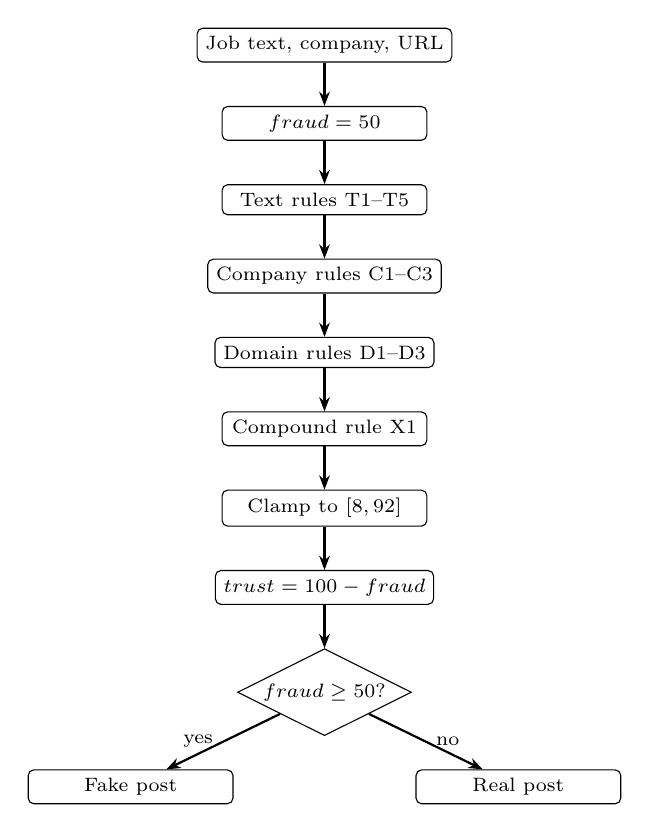
\begin{tikzpicture}[
  node distance=0.55cm and 0.4cm,
  box/.style={rectangle, draw, rounded corners=2pt, align=center, font=\scriptsize, inner sep=3pt, minimum width=2.6cm},
  dec/.style={diamond, draw, aspect=2, align=center, font=\scriptsize, inner sep=1pt},
  arr/.style={-{Stealth[length=1.8mm]}, thick}
]
\node[box] (in) {Job text, company, URL};
\node[box, below=of in] (base) {$\text{fraud}=50$};
\node[box, below=of base] (text) {Text rules T1--T5};
\node[box, below=of text] (co) {Company rules C1--C3};
\node[box, below=of co] (dom) {Domain rules D1--D3};
\node[box, below=of dom] (x1) {Compound rule X1};
\node[box, below=of x1] (clamp) {Clamp to $[8,92]$};
\node[box, below=of clamp] (trust) {$\text{trust}=100-\text{fraud}$};
\node[dec, below=of trust] (dec) {$\text{fraud}\geq 50$?};
\node[box, below left=0.7cm and 0.6cm of dec] (fake) {Fake post};
\node[box, below right=0.7cm and 0.6cm of dec] (real) {Real post};
\draw[arr] (in) -- (base);
\draw[arr] (base) -- (text);
\draw[arr] (text) -- (co);
\draw[arr] (co) -- (dom);
\draw[arr] (dom) -- (x1);
\draw[arr] (x1) -- (clamp);
\draw[arr] (clamp) -- (trust);
\draw[arr] (trust) -- (dec);
\draw[arr] (dec) -- node[left, font=\scriptsize]{yes} (fake);
\draw[arr] (dec) -- node[right, font=\scriptsize]{no} (real);
\end{tikzpicture}
\caption{Decision flow for the Phase-1 recruitment heuristic module.}
\label{fig:recruit_flow}
\end{figure}

We evaluated this baseline on 40 manually labeled posts (20 legitimate, 20 scam) with fixed threshold 50. Table~\ref{tab:recruit_eval} reports accuracy, precision, recall, and F1 treating scam as the positive class. Recall reached 100\% (all scams detected), but precision was 71.4\% because eight legitimate posts from employers outside the small whitelist were flagged---an expected whitelist bias that a learned model or registry lookup should address.

\begin{table}
\caption{Heuristic recruitment module evaluation ($N=40$, threshold 50).}
\label{tab:recruit_eval}
\begin{tabular}{|l|r|}
\hline
Metric & Value\\
\hline
Accuracy & 80.0\%\\
\hline
Precision (scam) & 71.4\%\\
\hline
Recall (scam) & 100.0\%\\
\hline
F1 (scam) & 83.3\%\\
\hline
TP / TN / FP / FN & 20 / 12 / 8 / 0\\
\hline
\end{tabular}
\end{table}

\paragraph{Section takeaway.}
Technical coverage is thin relative to impact; transformer fine-tuning plus explanation transfer from fake news is the most credible learned route, but any deployed system---heuristic or learned---must document rules or features, publish a decision flow, and report labeled-set metrics rather than accuracy alone.

\section{Explainable AI for Evidence-Aware Authenticity}
\label{sec:xai}

\subsection{Grad-CAM for Images}
Grad-CAM aggregates class gradients into late convolutional feature maps to generate a coarse heatmap. For face forgery, useful heat should concentrate on blending seams, facial inconsistency, or anomalous texture rather than irrelevant background. CNNs such as EfficientNet integrate Grad-CAM with modest runtime cost~\cite{r02,r07,r13,r39}.

\subsection{LIME and SHAP for Text}
LIME fits a simple local surrogate around a sample. SHAP attributes the prediction change to features under a cooperative-game interpretation. In practice, both surface tokens that push a label toward fake or real. They can disagree with each other and latch onto correlated wording; therefore, systems should store them as supporting evidence, not as causal ground truth~\cite{r26,r40,r29}.

\subsection{What Evidence-Aware Means Here}
We call a system evidence-aware when each prediction returns (i)~a threat-specific label, (ii)~a confidence score, and (iii)~an explanation artifact that a human reviewer can inspect---a Grad-CAM overlay, ranked token list, or both. Multi-threat frameworks become natural once each modality has a specialized detector and a shared audit log.

\section{Datasets and Evaluation Practices}
\label{sec:data}

\subsection{Common DeepFake Resources}
FaceForensics++, Celeb-DF, and related public sets dominate published image results~\cite{r18,r08,r09}. Many studies also add private or freshly generated samples to test newer synthesis methods~\cite{r04,r07}. Reporting only in-domain accuracy without cross-dataset checks overstates readiness for platform use.

\subsection{Fake News and Recruitment Corpora}
Fake news studies use multiple text and multimodal collections, and survey papers document the fragmentation of definitions and labels~\cite{r21,r31,r34}. Recruitment work often depends on EMSCAD-style job corpora or restricted institutional data~\cite{r38,r37}. Imbalance is the normal case: fraudulent posts are fewer, so accuracy alone can mislead.

\subsection{Metrics That Matter}
Accuracy, precision, recall, F1, and AUC appear almost everywhere. For authenticity platforms, one should also track the false-alarm rate under class skew, cross-dataset drop, latency for interactive review, and---when XAI is claimed---whether the explanation changes reviewer decisions~\cite{r19,r29}. The last metric is still rare.

\section{Comparative Summary and Reference Multi-Threat View}
\label{sec:compare}
Table~\ref{tab1} summarizes the technique families. Table~\ref{tab2} compares literature maturity by threat. Table~\ref{tab3} aligns modules with detectors and evidence methods.

\begin{table}
\caption{Representative technique families for digital deception detection.}
\label{tab1}
\begin{tabular}{|p{2.4cm}|p{2.3cm}|p{2.6cm}|p{2.6cm}|}
\hline
Family & Typical task & Main strength & Common weakness\\
\hline
EfficientNet / CNN & DeepFake images & Accuracy--cost trade-off & Cross-dataset drop\\
\hline
Vision transformer / hybrid & DeepFake image/video & Long-range cues & Compute and data hunger\\
\hline
Classical ML (TF--IDF, SVM) & News / job text & Simple, inspectable & Weak under paraphrase\\
\hline
BERT / graph--BERT & Fake news, recruitment & Contextual modelling & Opaque without XAI\\
\hline
Grad-CAM & Image explanation & Cheap visual evidence & Coarse localisation\\
\hline
LIME / SHAP & Text explanation & Local word rationale & Unstable; not causal proof\\
\hline
\end{tabular}
\end{table}

\begin{table}
\caption{Literature maturity by threat type.}
\label{tab2}
\begin{tabular}{|l|l|l|p{3.6cm}|}
\hline
Threat & Detector maturity & XAI maturity & Remarks\\
\hline
DeepFake images & High & Medium--high & Grad-CAM common; robustness fragile\\
\hline
Fake news & High & Medium & LIME/SHAP rising; multimodal growing\\
\hline
Recruitment scam & Low--medium & Low & Method transfer from fake news useful\\
\hline
\end{tabular}
\end{table}

\begin{table}
\caption{Evidence-aware module alignment suggested by the surveyed literature.}
\label{tab3}
\begin{tabular}{|p{2.3cm}|p{3.1cm}|p{2.4cm}|p{2.6cm}|}
\hline
Module & Detector suggestion & Evidence & Literature\\
\hline
Image authenticity & EfficientNetB0 / EfficientNet family & Grad-CAM & \cite{r02,r04,r07,r13,r39}\\
\hline
Fake news & BERT-style classifier & LIME / SHAP & \cite{r27,r26,r40}\\
\hline
Recruitment scam (literature) & BERT fine-tune + domain features & LIME / SHAP & \cite{r38,r37}\\
\hline
Recruitment scam (Phase-1 prototype) & Documented rule heuristics (Table~\ref{tab:recruit_rules}) & Rule indicators + token highlights & Eval.\ Table~\ref{tab:recruit_eval}\\
\hline
\end{tabular}
\end{table}

\noindent A practical multi-threat layout follows Table~\ref{tab3}: route images to an EfficientNet detector with Grad-CAM; route news and job text to a shared BERT text stack with LIME/SHAP; write every decision and artifact into one evidence log for later auditing. This is not claimed as a finished product architecture; it is a reading of where the literature already points.

\section{Open Challenges and Research Directions}
\label{sec:open}
\begin{enumerate}
\item \textbf{Cross-domain robustness.} Models strong on one generator or one news corpus often weaken elsewhere. Platform content is compressed, multilingual, and noisy. Cross-domain reporting should be mandatory for claims of deployability.
\item \textbf{Explanation fidelity.} Heatmaps and token ranks can appear credible while reflecting the wrong reasons. Quantitative stress tests of explanations~\cite{r19} deserve wider application.
\item \textbf{Multi-threat fusion.} Real incidents may combine a forged profile photograph with a deceptive job description. Joint pipelines and shared logs are still uncommon.
\item \textbf{Recruitment data scarcity.} Public hiring-fraud corpora are limited. Semi-supervised learning, careful augmentation, and privacy-aware label sharing are required.
\item \textbf{Human factors.} Adding XAI does not guarantee higher trust~\cite{r29}. Interface design and analyst workflow belong in the evaluation plan.
\item \textbf{Smart-service constraints.} Communication systems and digital-city services face latency, cost, and privacy limits. Lightweight EfficientNet variants and selective explanations are practical research targets.
\end{enumerate}

\section{Conclusion}
\label{sec:concl}
DeepFake, fake news, and recruitment fraud are usually studied separately, yet users encounter them on the same platforms. This survey linked the three threats through an evidence-aware authenticity lens. EfficientNet-family CNNs with Grad-CAM form a strong image pathway. BERT-family models with LIME/SHAP form a strong text path for both news and job advertisements. Recruitment fraud remains less prevalent than the other two areas but is operationally urgent. The clearest research opportunity is not another isolated high-accuracy classifier but a multi-threat framework that returns labels, confidence, and inspectable evidence together. Such frameworks are increasingly relevant for trustworthy communication platforms and safer digital services.

\begin{credits}
\subsubsection{\ackname}
The authors thank the Department of Artificial Intelligence \& Data Science, Parul Institute of Engineering \& Technology, Parul University, for support during this survey work.

\subsubsection{\discintname}
The authors have no competing interests to declare that are relevant to the content of this article.
\end{credits}
%
\begin{thebibliography}{99}

\bibitem{r01}
B. V. Moyo, T. Tuyikeze, F. Matsebula, et al: An AI-driven conceptual framework for detecting fake news and deepfake content: a systematic review. Frontiers in Artificial Intelligence, 9 (2026). \doi{10.3389/frai.2026.1737790}

\bibitem{r02}
M. Kumar, A. Kumar, V. Yadav, et al: A hybrid spatial–frequency attention-based algorithm using efficientnet for robust and interpretable deepfake detection. Scientific Reports, 16(1) (2026). \doi{10.1038/s41598-026-46086-9}

\bibitem{r03}
R. Chalehchaleh, R. Farahbakhsh, N. Crespi: Addressing data scarcity in multilingual fake news detection: an LLM-based dataset augmentation approach. Social Network Analysis and Mining, 15(1) (2025). \doi{10.1007/s13278-025-01505-z}

\bibitem{r04}
B. G. Deepa, C. K. Lokesh, D. Umamaheswari, et al: An enhanced deep learning framework for DeepFake detection using EfficientNet-B3 comparative evaluation of deep and machine learning techniques. Discover Computing, 29(1) (2026). \doi{10.1007/s10791-025-09890-x}

\bibitem{r05}
K. Omar, R. H. Sakr, M. F. Alrahmawy: An ensemble of CNNs with self-attention mechanism for DeepFake video detection. Neural Computing and Applications, 36(6), 2749–2765 (2024). \doi{10.1007/s00521-023-09196-3}

\bibitem{r06}
A. P. Magesh, S. S. M. Ramakrishnan, R. Arumuga Arun, et al: Building an efficient Deep Fake detection system using the recognition capabilities of convolutional neural networks and transformers. Discover Computing, 28(1) (2025). \doi{10.1007/s10791-025-09586-2}

\bibitem{r07}
F. Castro, V. Gattulli, D. Impedovo, et al: DeepDect: an explainable AI platform for face swapping and face generation DeepFake detection. Multimedia Tools and Applications, 85(5) (2026). \doi{10.1007/s11042-026-21672-1}

\bibitem{r08}
B. C. Soundarya, H. L. Gururaj: Deepfake detection: critical review of state-of-the-art approaches and future perspectives. Discover Applied Sciences, 8(2) (2026). \doi{10.1007/s42452-025-08174-9}

\bibitem{r09}
N. A. Bhat, K. J. Giri: DeepFake detection in images and videos: a survey on models, datasets, and evaluation metrics. Multimedia Tools and Applications, 85(3) (2026). \doi{10.1007/s11042-026-21365-9}

\bibitem{r10}
A. H. Soudy, O. Sayed, H. Tag-Elser, et al: Deepfake detection using convolutional vision transformers and convolutional neural networks. Neural Computing and Applications, 36(31), 19759–19775 (2024). \doi{10.1007/s00521-024-10181-7}

\bibitem{r11}
O. Pontorno, L. Guarnera, S. Battiato: DeepFeatureX-SN: Generalization of deepfake detection via contrastive learning. Multimedia Tools and Applications, 84(39), 47721–47740 (2025). \doi{10.1007/s11042-025-21060-1}

\bibitem{r12}
D. Javiya, G. Jethava, H. Parmar, et al: Enhancing deepfake detection with Adaptive-DCGAN and Lite-CNN: a novel approach to image classification. Discover Applied Sciences, 7(11) (2025). \doi{10.1007/s42452-025-07690-y}

\bibitem{r13}
N. Mansoor, A. I. Iliev: Explainable AI for DeepFake Detection. Applied Sciences, 15(2), 725 (2025). \doi{10.3390/app15020725}

\bibitem{r14}
M. S. Momin, A. Sufian, D. Barman, et al: Explainable deepfake detection across different modalities: An overview of methods and challenges. Image and Vision Computing, 163, 105738 (2025). \doi{10.1016/j.imavis.2025.105738}

\bibitem{r15}
S. Kaman, S. B. Javeriya, A. Makandar: Hybrid CNN-based detection of forged facial images using Gabor filters and local binary patterns. Discover Computing, 28(1) (2025). \doi{10.1007/s10791-025-09731-x}

\bibitem{r16}
Y. Sheng, Z. Zou, Z. Yu, et al: ID-insensitive deepfake detection model based on multi-attention mechanism. Scientific Reports, 15(1) (2025). \doi{10.1038/s41598-025-96254-6}

\bibitem{r17}
H. Duan, Q. Jiang, X. Jin, et al: Mf-net: multi-feature fusion network based on two-stream extraction and multi-scale enhancement for face forgery detection. Complex & Intelligent Systems, 11(1) (2025). \doi{10.1007/s40747-024-01634-6}

\bibitem{r18}
Y. Mirsky, W. Lee: The Creation and Detection of Deepfakes. ACM Computing Surveys, 54(1), 1–41 (2022). \doi{10.1145/3425780}

\bibitem{r19}
K. Tsigos, E. Apostolidis, S. Baxevanakis, et al: Towards Quantitative Evaluation of Explainable AI Methods for Deepfake Detection. 3rd ACM International Workshop on Multimedia AI against Disinformation, 37–45 (2024). \doi{10.1145/3643491.3660292}

\bibitem{r20}
F. Abbas, A. Taeihagh: Unmasking deepfakes: A systematic review of deepfake detection and generation techniques using artificial intelligence. Expert Systems with Applications, 252, 124260 (2024). \doi{10.1016/j.eswa.2024.124260}

\bibitem{r21}
J. Alghamdi, S. Luo, Y. Lin: A comprehensive survey on machine learning approaches for fake news detection. Multimedia Tools and Applications, 83(17), 51009–51067 (2023). \doi{10.1007/s11042-023-17470-8}

\bibitem{r22}
H. R. LekshmiAmmal, A. K. Madasamy: A reasoning based explainable multimodal fake news detection for low resource language using large language models and transformers. Journal of Big Data, 12(1) (2025). \doi{10.1186/s40537-025-01093-x}

\bibitem{r23}
L. A. Passos, D. Jodas, K. A. P. Costa, et al: A review of deep learning‐based approaches for deepfake content detection. Expert Systems, 41(8) (2024). \doi{10.1111/exsy.13570}

\bibitem{r24}
I. Ni’mah, R. Wijayanti, A. Santosa, et al: A simple contrastive embedding framework for low-resource fake news detection. Neural Computing and Applications, 37(26), 21407–21433 (2025). \doi{10.1007/s00521-025-11467-0}

\bibitem{r25}
S. Muthukumar, J. G. Fernandez, B. J. Ambika, et al: AI Based LSTM-BERT Model for False News Detection. Communications in Computer and Information Science, 124–134 (2026). \doi{10.1007/978-3-032-19318-6_12}

\bibitem{r26}
S. G. Sneha, A. Sen, S. Malik, et al: BiLSTM-LIME: integrating NLP and advanced machine learning models for fake news detection. Discover Artificial Intelligence, 6(1) (2026). \doi{10.1007/s44163-026-00852-w}

\bibitem{r27}
H. Rama Moorthy, N. J. Avinash, N. S. Krishnaraj Rao, et al: Dual stream graph augmented transformer model integrating BERT and GNNs for context aware fake news detection. Scientific Reports, 15(1) (2025). \doi{10.1038/s41598-025-05586-w}

\bibitem{r28}
M. E.Almandouh, M. F. Alrahmawy, M. Eisa, et al: Ensemble based high performance deep learning models for fake news detection. Scientific Reports, 14(1) (2024). \doi{10.1038/s41598-024-76286-0}

\bibitem{r29}
I. Bezzaoui, C. Stein, C. Weinhardt, et al: Explainable AI for online disinformation detection: Insights from a design science research project. Electronic Markets, 35(1) (2025). \doi{10.1007/s12525-025-00799-3}

\bibitem{r30}
S. Yakkundi, R. Patil, S. Sangani, et al: Exploring machine learning for fake news detection: techniques, tools, challenges, and future research directions. Discover Applied Sciences, 7(8) (2025). \doi{10.1007/s42452-025-07548-3}

\bibitem{r31}
F. A. Alshuwaier, F. A. Alsulaiman: Fake News Detection Using Machine Learning and Deep Learning Algorithms: A Comprehensive Review and Future Perspectives. Computers, 14(9), 394 (2025). \doi{10.3390/computers14090394}

\bibitem{r32}
C. Kumar, M. Bansal, M. A. Khan, et al: Graph-augmented transformer ensemble framework for robust and scalable fake news detection in social media ecosystems. Scientific Reports, 16(1) (2025). \doi{10.1038/s41598-025-31653-3}

\bibitem{r33}
G. K. M, K. S. Faizz Ahmad, S. G. Pamidimukkala, et al: Hybrid optimization driven fake news detection using reinforced transformer models. Scientific Reports, 15(1) (2025). \doi{10.1038/s41598-025-99936-3}

\bibitem{r34}
J. Lv, Y. Gao, L. Li, et al: Multi-modal fake news detection: A comprehensive survey on deep learning technology, advances, and challenges. Journal of King Saud University Computer and Information Sciences, 37(9) (2025). \doi{10.1007/s44443-025-00317-7}

\bibitem{r35}
A. B. Athira, S. D. Madhu Kumar, A. M. Chacko: Towards Smart Fake News Detection Through Explainable AI. arXiv:2207.11490 (2022). \doi{10.48550/arXiv.2207.11490}

\bibitem{r36}
B. S. Alqadi, S. A. Alsuhibany, S. N. Yousafzai, et al: Transfer learning driven fake news detection and classification using large language models. Scientific Reports, 15(1) (2025). \doi{10.1038/s41598-025-10670-2}

\bibitem{r37}
M. Naudé, K. J. Adebayo, R. Nanda: A machine learning approach to detecting fraudulent job types. AI & SOCIETY, 38(2), 1013–1024 (2023). \doi{10.1007/s00146-022-01469-0}

\bibitem{r38}
K. Taneja, J. Vashishtha, S. Ratnoo: Fraud-BERT: transformer based context aware online recruitment fraud detection. Discover Computing, 28(1) (2025). \doi{10.1007/s10791-025-09502-8}

\bibitem{r39}
DeepFake Detection Using CNN Models with Explainable AI Techniques: IEEE Access (2025). \doi{10.1109/ACCESS.2025.11135663}

\bibitem{r40}
X. Men, V. Y. Mariano: Explainable Fake News Detection Based on BERT and SHAP Applied to COVID-19. International Journal of Modern Education and Computer Science, 16(1), 11–22 (2024). \doi{10.5815/ijmecs.2024.01.02}

\end{thebibliography}
\end{document}
